\begin{figure}[H]
\centering

\includegraphics[width=\textwidth]{100b99d2acd92e338d74f6882feacff.jpg}
% \caption{}
\label{}
\end{figure}

\section{增加复制构造函数和重载赋值运算符}

\begin{figure}[H]
\centering
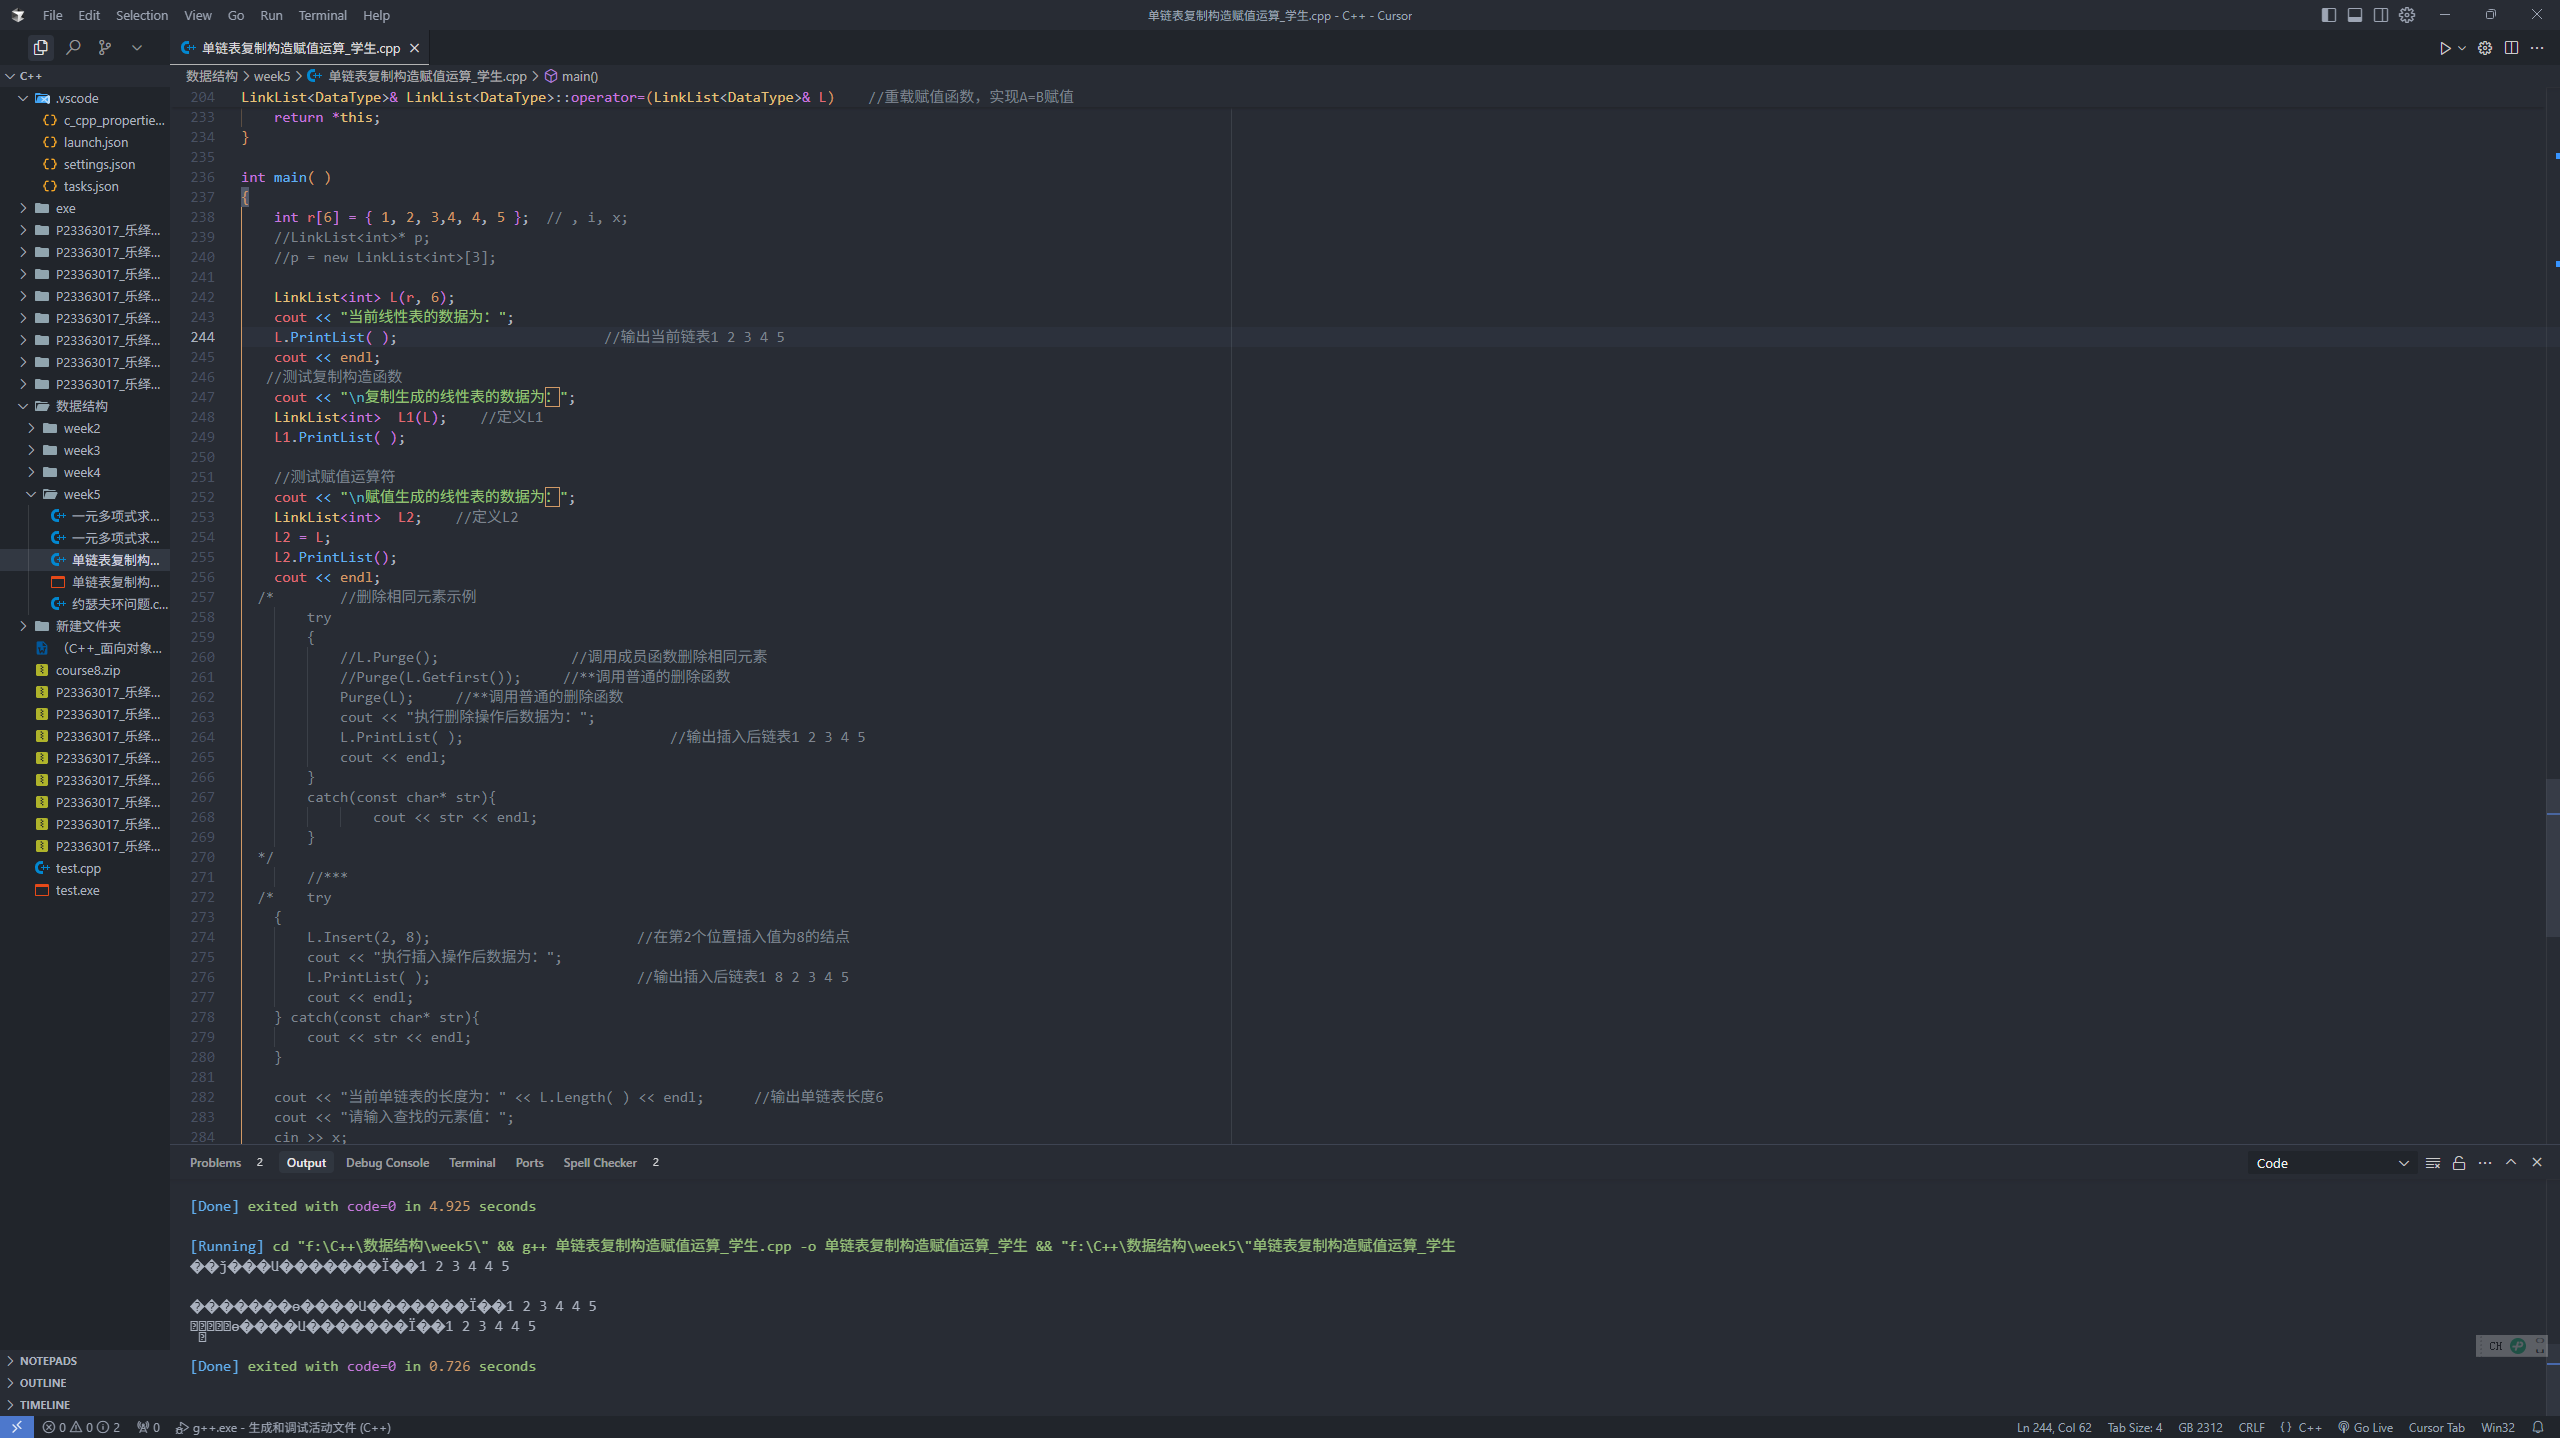
\includegraphics[width=\textwidth]{实验报告5-2025033121.png}
% \caption{}
\label{}
\end{figure}

\begin{lstlisting}[language=C++]
template <class DataType>

LinkList<DataType>::LinkList(const LinkList<DataType> &L)    //复制构造函数,带头节点

{

    first = new Node<DataType>;

    first->next = NULL;

    Node<DataType> *p = L.first->next;

    Node<DataType> *r = first;

    while(p != NULL)

    {

        Node<DataType> *s = new Node<DataType>;

        s->data = p->data;

        s->next = NULL;

        r->next = s;

        r = s;

        p = p->next;

    }

    r->next = NULL;

}

  

template <class DataType>

LinkList<DataType>& LinkList<DataType>::operator=(LinkList<DataType>& L)    //重载赋值函数,实现A=B赋值

{

    // 检查自赋值

    if (this == &L)

        return *this;

    // 释放原有链表内存

    Node<DataType> *p = first->next;

    while (p != NULL)

    {

        Node<DataType> *temp = p;

        p = p->next;

        delete temp;

    }

    // 复制L的内容

    p = L.first->next;

    Node<DataType> *r = first;

    while (p != NULL)

    {

        Node<DataType> *s = new Node<DataType>;

        s->data = p->data;

        s->next = NULL;

        r->next = s;

        r = s;

        p = p->next;

    }

    r->next = NULL;

    return *this;

}
\end{lstlisting}
\section{一元多项式求和,数据从文件中读入,考虑运算符重载}

\begin{figure}[H]
\centering
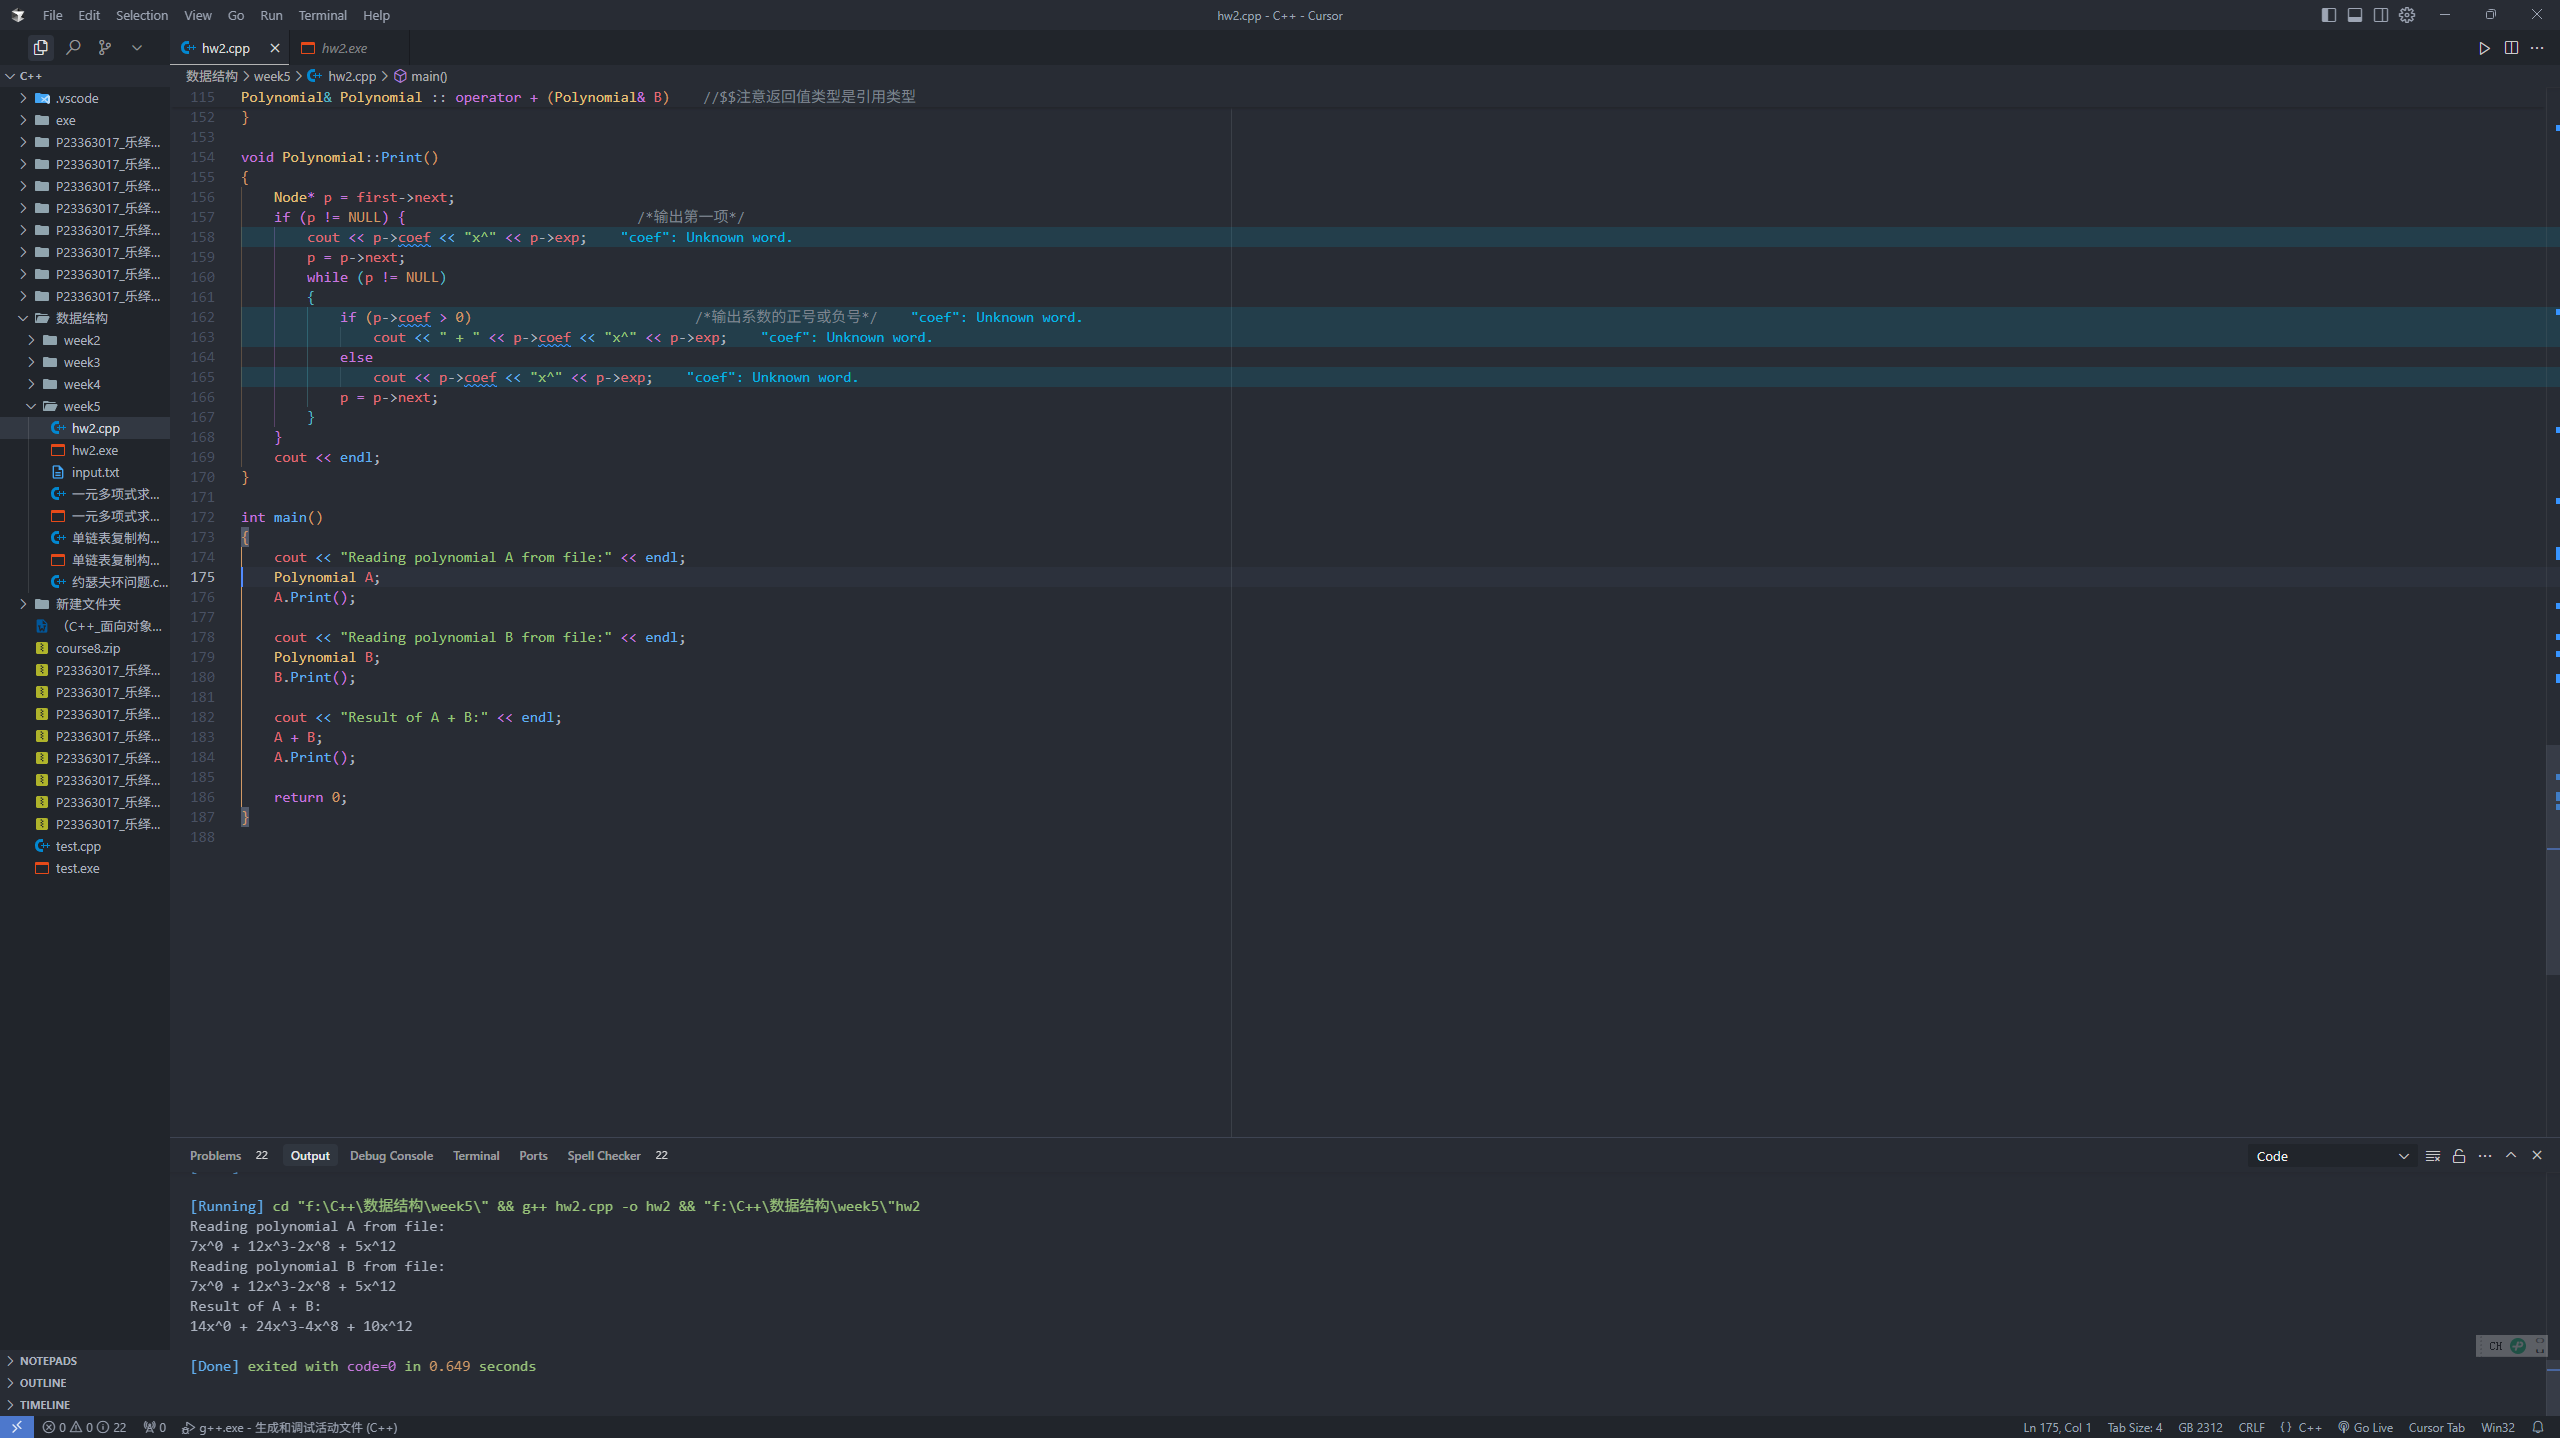
\includegraphics[width=\textwidth]{1-实验报告5-2025033121.png}
% \caption{}
\label{}
\end{figure}

\begin{lstlisting}[language=C++]
/**************************************

   对应教材 2.7.2节,一元多项式求和

***************************************/

#include <iostream>      

#include <fstream>

using namespace std;

  

struct Node                                  //定义多项式链表的结点

{

    int coef, exp;                          // coef表示系数,exp表示指数

    Node* next;

};

  

class Polynomial

{

public:

    Polynomial();                          //构造函数

    ~Polynomial();                         //析构函数,同单链表析构函数

    Polynomial(const Polynomial& B);          //拷贝构造函数

    Polynomial & operator=(Polynomial &L);  //重载赋值运算符

    Polynomial & operator + (Polynomial& B);   //重载运算法,多项式相加

    void Print();                           //打印一元多项式

private:

    Node* first;

};

  

Polynomial::~Polynomial()

{

    Node* q = NULL;

    while (first != NULL)        //释放单链表的每一个结点的存储空间

    {

        q = first;                 //暂存被释放结点

        first = first->next;         // first指向被释放结点的下一个结点

        delete q;

    }

}

  

/*Polynomial::Polynomial(const Polynomial& B) {

    first = B.first;

}

*/

//复制构造函数的算法

//template <class DataType>

//LinkList<DataType>::LinkList(LinkList<DataType>& L)    //复制构造函数,带头节点

Polynomial::Polynomial(const Polynomial & B)

{

    Node* s, *srcptr = B.first;              //被复制表的头节点

    Node* destptr = new Node;

    first = destptr;            //$$$特别注意这里要把first指向新生成的节点

    while (srcptr->next != NULL) {     //逐个节点复制

          s = new Node;         //生成新节点

          s->coef = srcptr->next->coef;

          s->exp = srcptr->next->exp;

          destptr->next = s;

          destptr = destptr->next;

          srcptr = srcptr->next;

  

    }

    destptr->next = NULL;//最后一个节点的next要置空  

}

  
  

//重载赋值运算符的算法

//template <class DataType>

//LinkList<DataType>& LinkList<DataType>::operator=(LinkList<DataType>& L)    //重载赋值函数,实现A=B赋值

Polynomial & Polynomial::operator=(Polynomial &L)  //例如:LA=L

{

    Node * s,*q, * srcptr = L.first;              //被复制表L的头节点

    Node * destptr =first ;   //$$利用被赋值链表的头节点

    if (first == L.first) return *this;   //$$如果自己赋值给自己,比如:A=A,直接返回

    s = first->next;

    while (s != NULL) {     //$$释放被赋值链表以前的空间

        q = s; s = s->next;

        delete q;

    };

    while (srcptr->next != NULL) {     //逐个节点复制

          s = new Node ;         //生成新节点

          s->coef = srcptr->next->coef;

          s->exp = srcptr->next->exp;

          destptr->next = s;

          destptr = destptr->next;

          srcptr = srcptr->next;

  

    }

    destptr->next = NULL; //最后一个节点的next要置空  

    return *this;     //返回赋值结果

}

  
  
  

Polynomial::Polynomial()

{

    Node* r = NULL, * s = NULL;

    int coef, exp;

    first = new Node;                          //create head node

    r = first; r->next = NULL;             //build linked list using tail insertion

    // 从文件读取数据

    ifstream inFile("input.txt");

    if (!inFile) {

        cout << "无法打开输入文件!" << endl;

        return;

    }

    while (inFile >> coef >> exp) {

        if (coef == 0 && exp == 0) break;

        s = new Node; s->coef = coef; s->exp = exp;

        r->next = s; r = s;

    }

    r->next = NULL;

    inFile.close();

}

  

Polynomial& Polynomial :: operator + (Polynomial& B)    //$$注意返回值类型是引用类型

{

    Node* pre = first, * p = pre->next;               //工作指针pre和p初始化

    Node* qre = B.first, * q = qre->next;             //工作指针qre和q初始化

    Node* qtemp = NULL;

    while (p != NULL && q != NULL)

    {

        if (p->exp < q->exp) {                     //第1种情况

            pre = p; p = p->next;

        }

        else if (p->exp > q->exp) {                 //第2种情况

            qtemp = q->next;

            pre->next = q;                     //将结点q插入到结点p之前

            q->next = p;

            pre = q;     //$$

            q = qtemp;

            //pre = q;

            qre->next = q;

        }

        else {                             //第3种情况

            p->coef = p->coef + q->coef;

            if (p->coef == 0) {                //系数相加为0,则删除结点p

                pre->next = p->next;

                delete p;

                p = pre->next;

            }

            else {                          //系数不为0

                pre = p; p = p->next;

            }

            qre->next = q->next;             //第3种情况都要删除结点q

            delete q;

            q = qre->next;

        }

    }

    if (q != NULL) pre->next = q;          //将结点q链接在第一个单链表的后面

    B.first->next = NULL;

    return *this;

}

  

void Polynomial::Print()

{

    Node* p = first->next;

    if (p != NULL) {                            /*输出第一项*/

        cout << p->coef << "x^" << p->exp;

        p = p->next;

        while (p != NULL)

        {

            if (p->coef > 0)                           /*输出系数的正号或负号*/

                cout << " + " << p->coef << "x^" << p->exp;

            else

                cout << p->coef << "x^" << p->exp;

            p = p->next;

        }

    }

    cout << endl;

}

  

int main()

{

    cout << "Reading polynomial A from file:" << endl;

    Polynomial A;

    A.Print();

    cout << "Reading polynomial B from file:" << endl;

    Polynomial B;

    B.Print();

    cout << "Result of A + B:" << endl;

    A + B;

    A.Print();

    return 0;

}
\end{lstlisting}
\section{3. 用有序链表实现集合的判等、交、并、差等基本运算。要考虑算法时间和空间性能。}

\begin{figure}[H]
\centering
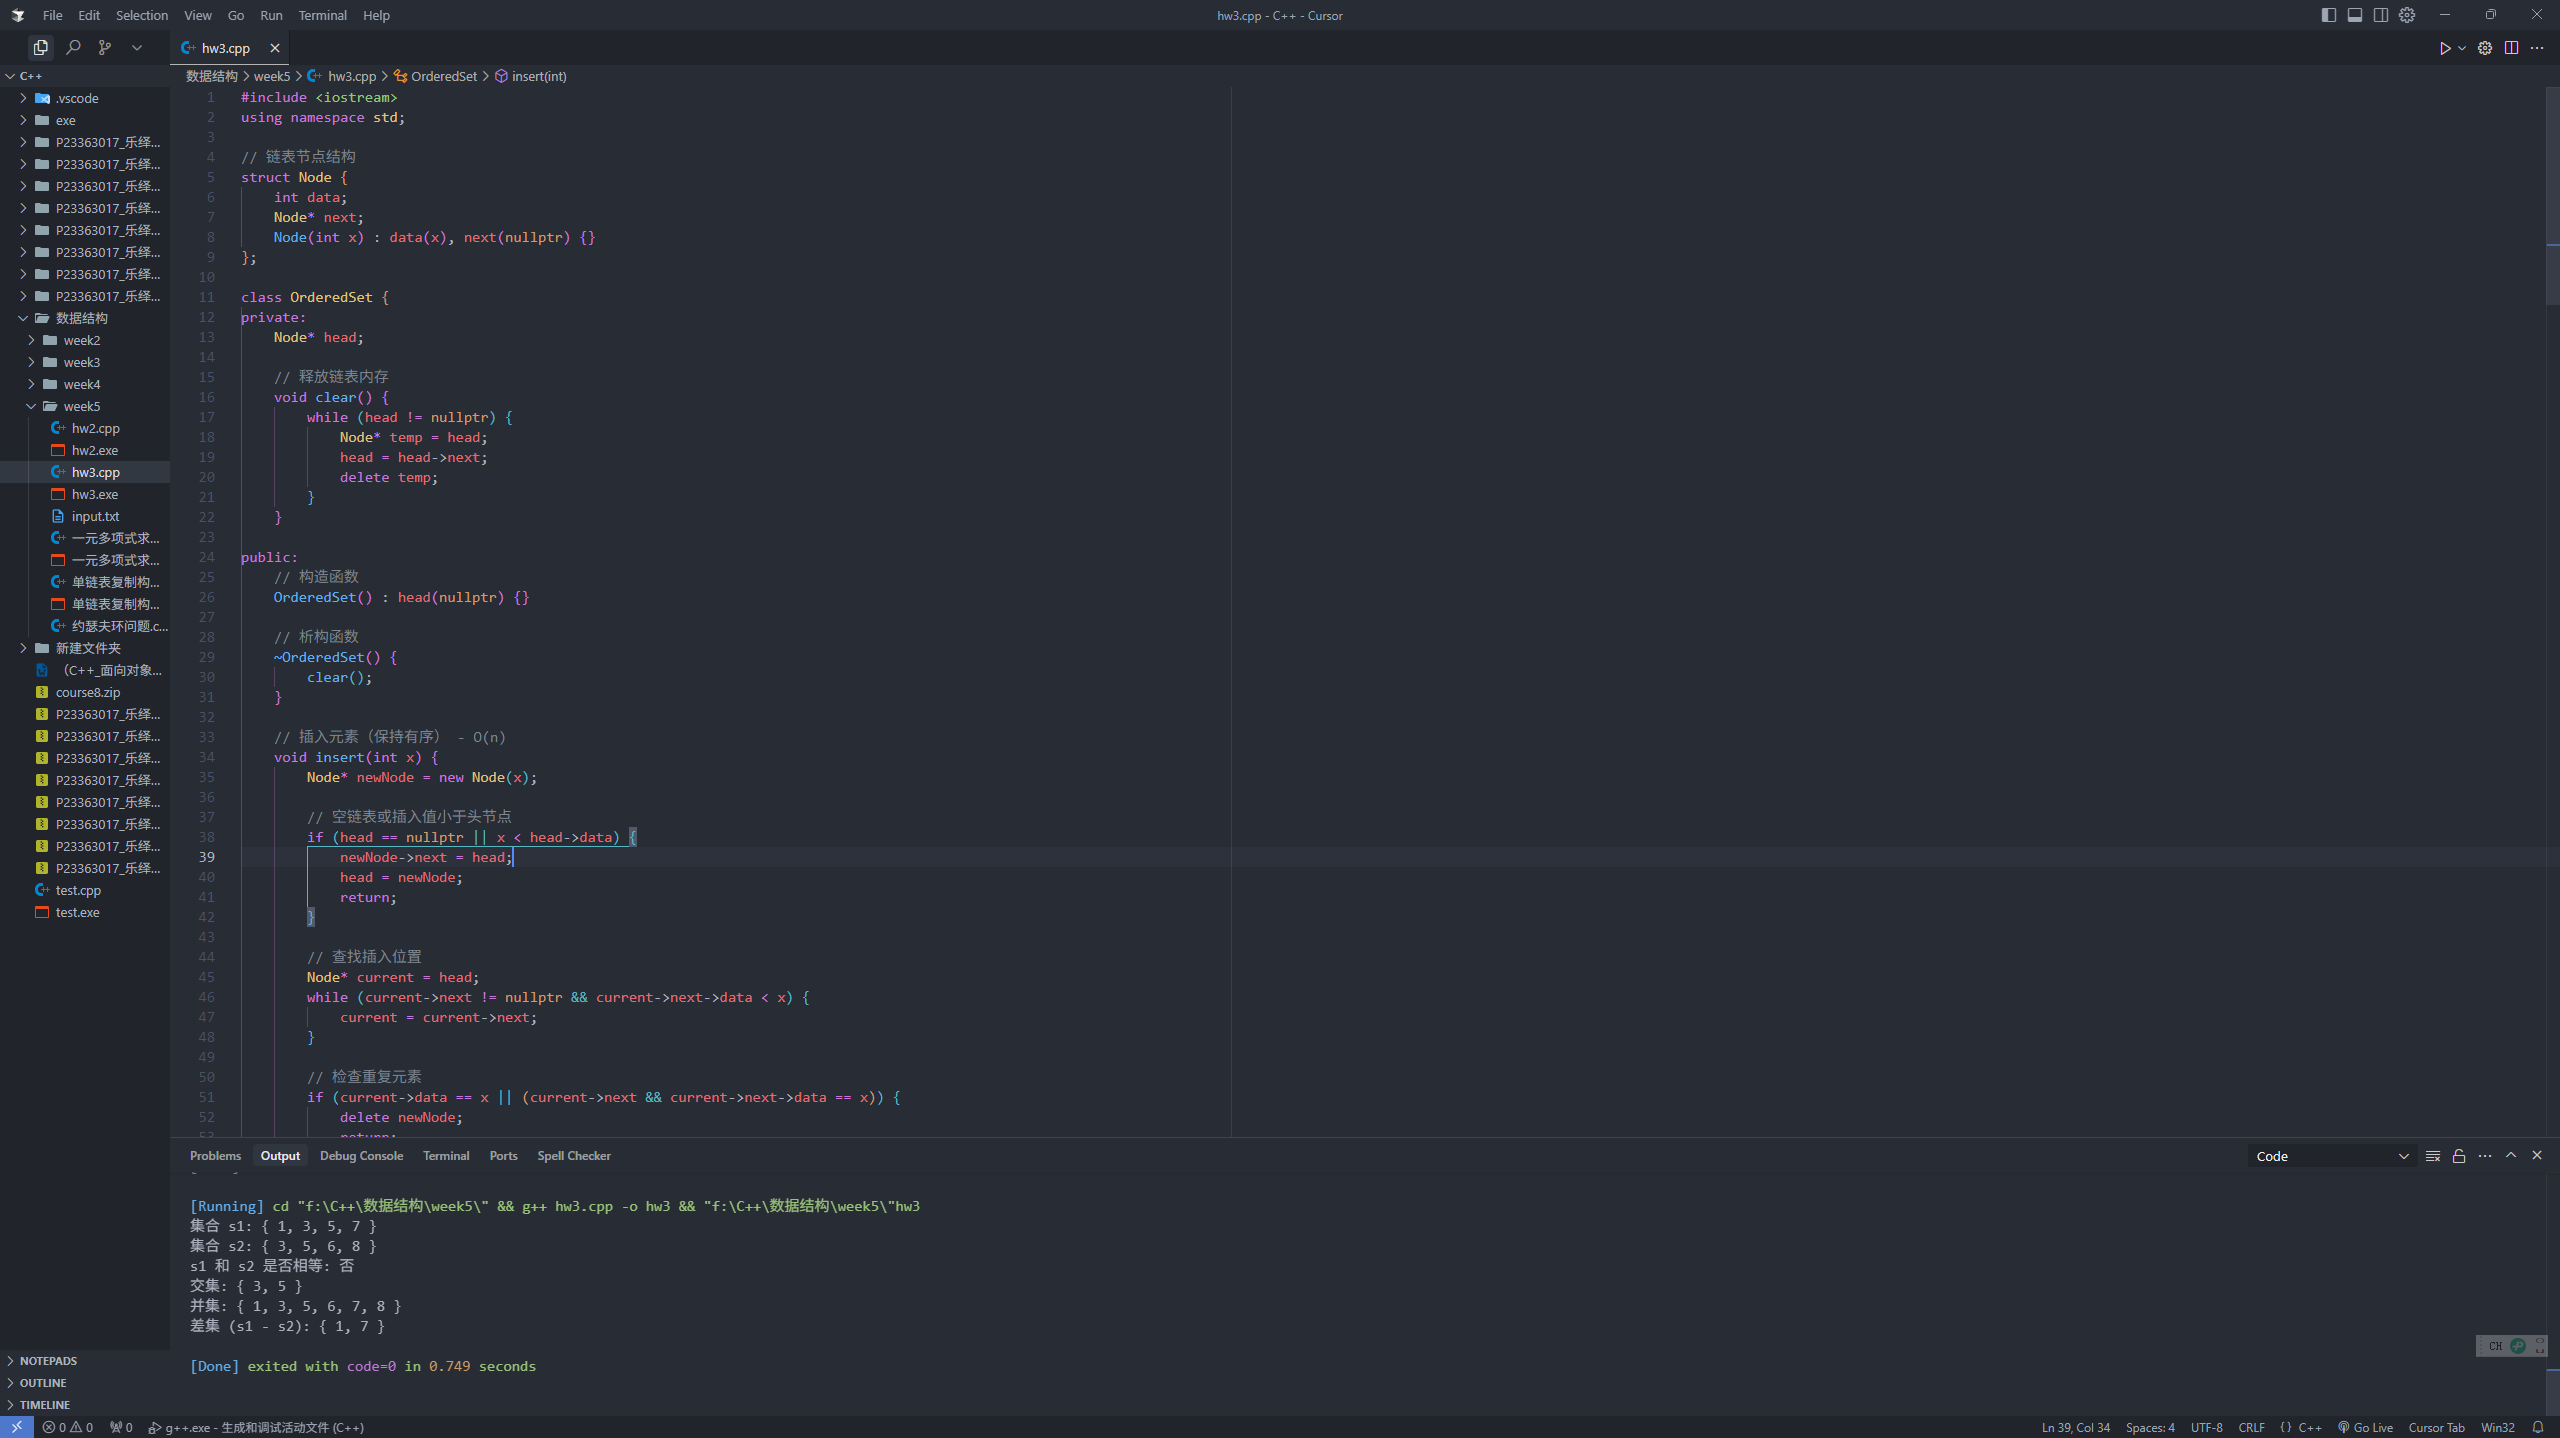
\includegraphics[width=\textwidth]{实验报告5-2025033122.png}
% \caption{}
\label{}
\end{figure}

判等、交、并、差运算的时间复杂度都为 $O(n)$.

\begin{lstlisting}[language=C++]
#include <iostream>

using namespace std;

  

// 链表节点结构

struct Node {

    int data;

    Node* next;

    Node(int x) : data(x), next(nullptr) {}

};

  

class OrderedSet {

private:

    Node* head;

  

    // 释放链表内存

    void clear() {

        while (head != nullptr) {

            Node* temp = head;

            head = head->next;

            delete temp;

        }

    }

  

public:

    // 构造函数

    OrderedSet() : head(nullptr) {}

    // 析构函数

    ~OrderedSet() {

        clear();

    }

  

    // 插入元素(保持有序) - O(n)

    void insert(int x) {

        Node* newNode = new Node(x);

        // 空链表或插入值小于头节点

        if (head == nullptr || x < head->data) {

            newNode->next = head;

            head = newNode;

            return;

        }

  

        // 查找插入位置

        Node* current = head;

        while (current->next != nullptr && current->next->data < x) {

            current = current->next;

        }

  

        // 检查重复元素

        if (current->data == x || (current->next && current->next->data == x)) {

            delete newNode;

            return;

        }

  

        newNode->next = current->next;

        current->next = newNode;

    }

  

    // 判等运算 - O(n)

    bool equals(const OrderedSet& other) const {

        Node* p1 = head;

        Node* p2 = other.head;

  

        while (p1 && p2) {

            if (p1->data != p2->data) return false;

            p1 = p1->next;

            p2 = p2->next;

        }

  

        return p1 == nullptr && p2 == nullptr;

    }

  

    // 交集运算 - O(n)

    OrderedSet intersection(const OrderedSet& other) const {

        OrderedSet result;

        Node* p1 = head;

        Node* p2 = other.head;

  

        while (p1 && p2) {

            if (p1->data < p2->data) {

                p1 = p1->next;

            } else if (p2->data < p1->data) {

                p2 = p2->next;

            } else {

                result.insert(p1->data);

                p1 = p1->next;

                p2 = p2->next;

            }

        }

  

        return result;

    }

  

    // 并集运算 - O(n)

    OrderedSet union_with(const OrderedSet& other) const {

        OrderedSet result;

        Node* p1 = head;

        Node* p2 = other.head;

  

        while (p1 && p2) {

            if (p1->data < p2->data) {

                result.insert(p1->data);

                p1 = p1->next;

            } else if (p2->data < p1->data) {

                result.insert(p2->data);

                p2 = p2->next;

            } else {

                result.insert(p1->data);

                p1 = p1->next;

                p2 = p2->next;

            }

        }

  

        // 处理剩余元素

        while (p1) {

            result.insert(p1->data);

            p1 = p1->next;

        }

        while (p2) {

            result.insert(p2->data);

            p2 = p2->next;

        }

  

        return result;

    }

  

    // 差集运算 - O(n)

    OrderedSet difference(const OrderedSet& other) const {

        OrderedSet result;

        Node* p1 = head;

        Node* p2 = other.head;

  

        while (p1 && p2) {

            if (p1->data < p2->data) {

                result.insert(p1->data);

                p1 = p1->next;

            } else if (p2->data < p1->data) {

                p2 = p2->next;

            } else {

                p1 = p1->next;

                p2 = p2->next;

            }

        }

  

        // 添加剩余元素

        while (p1) {

            result.insert(p1->data);

            p1 = p1->next;

        }

  

        return result;

    }

  

    // 打印集合

    void print() const {

        Node* current = head;

        cout << "{ ";

        while (current) {

            cout << current->data;

            if (current->next) cout << ", ";

            current = current->next;

        }

        cout << " }" << endl;

    }

};

  

// 测试代码

int main() {

    OrderedSet s1, s2;

    // 插入测试数据

    s1.insert(1);

    s1.insert(3);

    s1.insert(5);

    s1.insert(7);

    s2.insert(3);

    s2.insert(5);

    s2.insert(6);

    s2.insert(8);

  

    cout << "集合 s1: ";

    s1.print();

    cout << "集合 s2: ";

    s2.print();

  

    cout << "s1 和 s2 是否相等: " << (s1.equals(s2) ? "是" : "否") << endl;

  

    cout << "交集: ";

    s1.intersection(s2).print();

  

    cout << "并集: ";

    s1.union_with(s2).print();

  

    cout << "差集 (s1 - s2): ";

    s1.difference(s2).print();

  

    return 0;

}
\end{lstlisting}
\section{用不带头结点的单循环链表,实现约瑟夫环问题}

\begin{figure}[H]
\centering
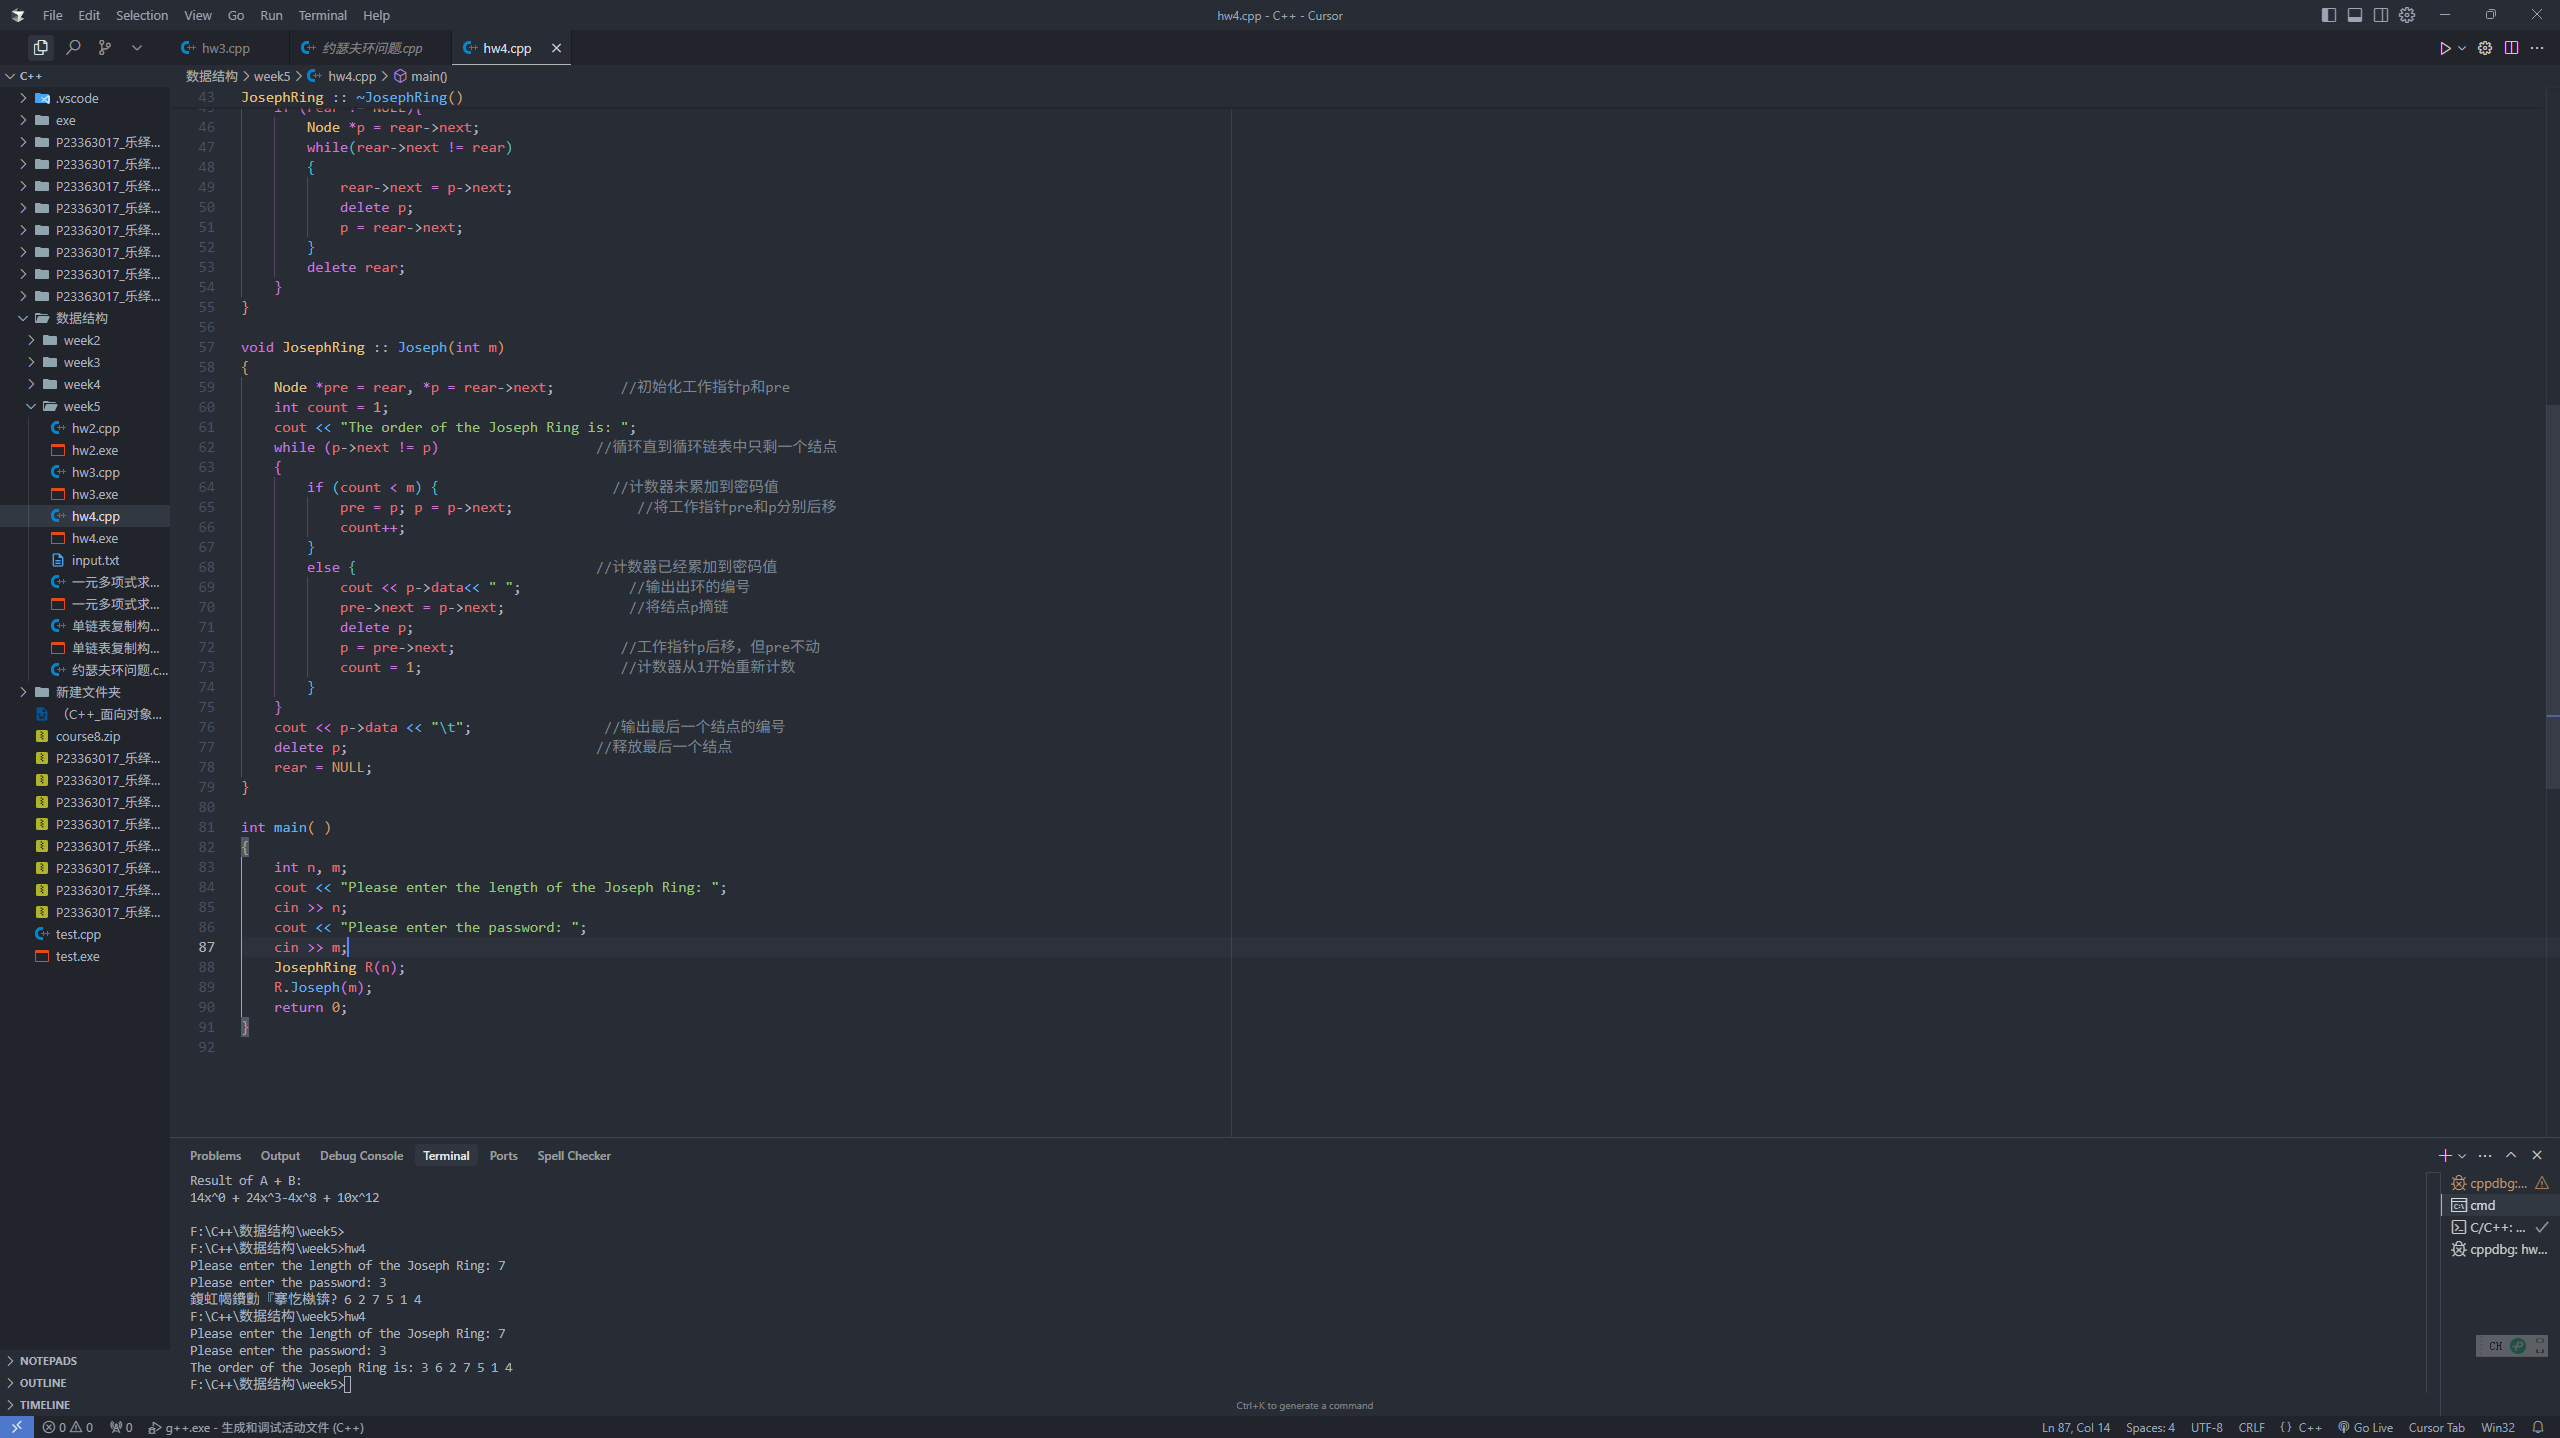
\includegraphics[width=\textwidth]{1-实验报告5-2025033122.png}
% \caption{}
\label{}
\end{figure}

\begin{lstlisting}[language=C++]
/**************************************

     对应教材 2.7.1节,约瑟夫环问题

***************************************/

#include <iostream>              

using namespace std;

  

struct Node                            //定义约瑟夫环的结点Node

{

    int data;

    struct Node *next;

};

  

class JosephRing

{

public:

    JosephRing( );                      //构造函数,初始化空循环链表

    JosephRing(int n);                 //构造函数,初始化n个结点的环

    ~JosephRing( );                    //析构函数,同单链表析构函数

    void Joseph(int m);                //密码为m,打印出环的顺序

private:

    Node *rear;

};

  

JosephRing :: JosephRing( )

{

    rear = NULL;

}

JosephRing :: JosephRing(int n)                            

{

    Node *s = NULL;  

    rear = new Node;    

    rear->data = 1; rear->next = rear;     //建立长度为1的循环单链表

    for (int i = 2; i <= n; i++)           //依次插入数据域为2、3、…、n的结点

    {

        s = new Node; s->data = i;

        s->next = rear->next;               //将结点s插入尾结点rear的后面

        rear->next = s;

        rear = s;                         //指针rear指向当前的尾结点

    }

}

  

JosephRing :: ~JosephRing()

{

    if (rear != NULL){

        Node *p = rear->next;

        while(rear->next != rear)

        {

            rear->next = p->next;

            delete p;

            p = rear->next;

        }

        delete rear;

    }

}

  

void JosephRing :: Joseph(int m)  

{    

    Node *pre = rear, *p = rear->next;        //初始化工作指针p和pre

    int count = 1;                        

    cout << "The order of the Joseph Ring is: ";

    while (p->next != p)                   //循环直到循环链表中只剩一个结点

    {

        if (count < m) {                     //计数器未累加到密码值

            pre = p; p = p->next;               //将工作指针pre和p分别后移

            count++;                                    

        }

        else {                             //计数器已经累加到密码值

            cout << p->data<< " ";             //输出出环的编号

            pre->next = p->next;               //将结点p摘链

            delete p;                    

            p = pre->next;                    //工作指针p后移,但pre不动

            count = 1;                        //计数器从1开始重新计数

        }

    }

    cout << p->data << "\t";                //输出最后一个结点的编号

    delete p;                              //释放最后一个结点

    rear = NULL;

}

  

int main( )

{

    int n, m;

    cout << "Please enter the length of the Joseph Ring: ";  

    cin >> n;

    cout << "Please enter the password: ";            

    cin >> m;

    JosephRing R(n);

    R.Joseph(m);

    return 0;                  

}
\end{lstlisting}